\section{Analyse af anvendelsesområdet}\label{sec:anvendelses}
Dette afsnit tager udgangspunkt i metoder fra ''Objektorienteret Analyse og Design'' og benytter disse til at analyserer anvendelsområdet, dette omfatter brug af systemet, funktioner i systemet samt grænsefladen der er tilknyttet.\citep{OOA&D2001}
Afsnittet skal give et overblik over funktionaliteten af systemet, samt formidle hvordan brugeren interagerer med systemet.

\subsection{Brug}
Denne del af analysen har til formål at fastlægge interaktion mellem systemet og aktører.
Dette gøres ved at identificere brugsmønstre for aktørerernes aktioner i systemet.
\subsubsection*{Aktører}
I dette IT-system er der blevet identificeret to aktører.
Den første værende datakilden, eTilbudsaviss API, hvor tilbudende hentes fra og den anden værende de brugere, som benytter systemet.
For disse to aktører er der således udarbejdet en aktørtabel \myref{aktortabel}, der giver overblik over hvilke brugsmønstre der er, samt hvilke aktører der er relevante for disse.

\begin{table}[h]
\centering
    \colorlet{shadecolor}{gray!40}
    \rowcolors{1}{white}{shadecolor}
\begin{tabular}{rcc}
%\hline
				    & Bruger               		& eTilbudsavis  \\ \hline
Login               & \cmark                    & 		 		\\
Listehåndtering     & \cmark                    & 		 		\\
Søgning             & \cmark                    & 				\\
Indstil præferencer & \cmark                    & 				\\
Vurder opskrift     & \cmark                    &  	   			\\
Se anbefalinger     & \cmark                    & 				\\
Hent tilbud         &  						    & \cmark 		\\ \hline
\end{tabular}
\caption{Aktørtabel. Viser hvilke aktører er involveret i hvilke brugsmønstre}\label{aktortabel}
\end{table}

\subsubsection*{Bruger}

\textbf{Formål:} En person, som ønsker at bruge en eller flere af IT-systemets funktionaliteter, til at hjælpe med planlægning af mad og indkøb.

\textbf{Karakteristik:} Systemets brugere har meget varierende erfaring med IT-systemer, samt er bredt ud over mange forskellige aldersgrupper, majoriteten er dog mellem 18 - 30 år og har middel erfaring med IT.

\textbf{Eksempler:}Bruger A er en 21-årig universitetsstuderende, som for nyligt er flyttet hjemmefra. A har meget erfaring med IT, og bruger det dagligt til at navigere rundt på internettet.
A har let ved at navigere rundt i systemet og bruge dets funktionaliteter til at lave besparelser på det allerede lave budget, samt at undgå at få pasta med ketchup til aftensmad hver dag.

Bruger B er en 47-årig familiefar, der kun har smartphone, da dette er arbejdstelefonen givet af hans arbejdsgiver.
B benytter systemet til at handle ind på vej hjem fra arbejde, hvor indkøbslisten lavet af konen eller datteren bruges som guide i supermarkedet.
B vil således gerne kunne tilgå listen fra telefonen, så der ikke er behov for at køre hjem og hente den på papirsformat.

\subsubsection*{eTilbudsavis}

\textbf{Formål:} eTilbudsavis har til formål at gøre tilbudsdata tilgængelig for systemet, dette sker igennem API.
Dette giver information om navnet på tilbudet, pris, periode, butik og meget andet.
Da dataene der hentes igennem API'et kan være af meget svingende kvalitet, filtreres det, så kun forståeligt tilbudsdata kommer igennem.

\textbf{Karakteristik:} eTilbudsavis er pålidelig med dataene der sendes, kvaliteten af dataene kan dog svinge meget, og eTilbudsavis tilbyder ingen fleksibilitet i dets arbejde, hvilket resulterer i noget ubrugeligt data som filtreres fra.

\textbf{Eksempel:} eTilbudsavis gør 2.000 tilbud tilgængelig, heri er nogle på et format der ikke klargøre hvad der er på tilbud, men blot giver en række mærkenavne som er på tilbud.
En sådan uforståelig række bliver filtreret ud såvel som andre uforståelige tilbud, og systemet ender tilbage med 1.337 brugbare tilbud, der kan vises til brugeren.

\subsubsection*{Brugsmønstre}
For en yderligere beskrivelse af de funktionaliteter i systemet, som vedrører en given aktør, modelleres en række brugsmønstre, dette er de samme brugsmønstre som ses i aktørtabellen i \myref{aktortabel}.
Hver enkelt af disse mønstre vil blive beskrevet igennem en brugsmønstrespecifikation.
Det er ikke alle mønstre som ses på denne liste, nogle af disse er sammentrækninger af flere andre mønstre, som alene virker simple og repetitive at beskrive.
Andre er udeladt da de ikke passer helt ind i en sammentrækning, men variationen fra det mønster og andre brugsmønstre ellers beskrevet, er så minimal, at mønstret er anset som værende ubetydeligt at beskrive.

\subsubsection*{Brugeridentifikation}
\textit{Brugsmønster:} Brugeridentifikation sker ved at en bruger logger ind i systemet.
Brugeren vil blive præsenteret for en side hvor, e-mail og password kan indtastes.
Herefter godkender eller afviser systemet den indtastede data og håndterer resultatet, enten ved at logge brugeren ind, eller ved at give en fejlbesked.
Alternativt kan brugeren oprette en ny konto i systemet, ved oplysning af navn e-mail og password.
Hvis du ikke er logget ind i systemet kan du ikke tilgå systemets funktionaliteter.

\textit{Objekter:} Person.

\textit{Funktioner:} Registrer bruger, Log ind, Log ud.

\subsubsection*{Listehåndtering}
\textbf{Brugsmønster:} Dette brugsmønster dækker over indkøbslisten såvel som overvågningslisten.
Brugeren kan inden for listens brugsmønstre tilgå funktionaliteterne i vilkårlig rækkefølge, givet der er oprettet en liste på forhånd.
En bruger kan oprette, dele og slette sine egne indkøbslister.
Hvis en liste er delt med andre og prøver at slette denne, forlader brugeren listen frem for at slette den.
Overvågningslisten på den anden hånd, eksisterer altid og kan hverken oprettes eller slettes.
Brugeren kan på begge lister tilføje eller fjerne en vare.
Varerne på overvågningslisten er varer som brugeren er interesserede i at få tilbud om.
Når en vare på denne liste kommer på tilbud modtager brugeren en notifikation derom.
Ved indkøbslisten er der tre funktionaliteter til at tilføje ting til listen.
Man kan tilføje ingredienser fra en opskrift.
Ydermere kan en bruger aftjekke eller fjerne varer fra listen.

\textbf{Objekter:} Indkøbsliste, Overvågningsliste, Varer, Tilbud, Personer, Opskrifter.

\textbf{Funktioner:} Opret liste, Fjern Indkøbsliste, Tilføj til liste, Fjern fra liste, Aftjek på indkøbsliste, Del liste, Forlad Indkøbsliste.

\subsubsection*{Søgning}
\textbf{Brugsmønster:} Brugeren kan søge efter varer, hvorefter systemet filtrerer efter søgestrengen for at finde relevante resultater.
Dette brugsmønster benyttes flere steder, både til at søge på tilbud til sine varer, såvel som opskrifter.


\textbf{Objekter:} Vare, Tilbud, Opskrifter.

\textbf{Funktioner:} Søg efter tilbud, Søg efter opskrifter.

\subsubsection*{Tilpas præferencer}
\textbf{Brugsmønster:} 
Brugere i systemet har mulighed for at fravælge madvarer eller butikker, som vises i programmet.

\textbf{Objekter:} Varer.

\textbf{Funktioner:} Sæt Præferencer, Filtrer efter præferencer.

\subsubsection*{Opskrifts håndtering}
\textbf{Brugsmønster:}
Brugeren kan interagere med opskrifter på forskellig vis. 
Som bruger har man mulighed for at oprette, klone, ændre, slette og vurdere opskrifter.
Når en opskrift oprettes vil brugeren bedes tilføje instruktioner, tid og ingredienser.
En bruger vil have mulighed for at ændre i sine egne opskrifter, og ligeledes kunne kopiere andres opskrifter og derefter tilføje ændringer i disse.
Fra ingredienslisten på en opskrift kan brugerne tilføje en eller flere varer til deres indkøbslister, samt skalere ingredienslisten til et bestemt antal personer, så brugerne får købt den rigtige mængde.
Brugerne har også mulighed for at vurdere opskrifter, ud fra brugerens vurderinger, vil systemet anbefale nye opskrifter til brugeren.

\textbf{Objekter:} Opskrift, Vurdering, liste af vurderinger, varer, indkøbsliste.

\textbf{Funktioner:} Se opskrift, oprette opskrift, ændre opskrift, klone opskrift, vurder opskrift, tilføj vare til liste, skalering af opskrift, slette opskrift.

%\subsubsection*{Vurder}
%\textbf{Brugsmønster:}
%Efter en opskrift er vurderet, kan andre brugere se den gennemsnitlige vurdering af en opskrift, og de brugere som har vurderet opskrifter, vil få anbefalet opskrifter som ligner.
%
%\textbf{Objekter:} Opskrift, Vurderinger, Liste af vurderinger.
%
%\textbf{Funktioner:} Vurder opskrift.

\subsubsection*{Se anbefalinger}
\textbf{Brugsmønster:} Brugeren kan se foreslåede opskrifter ud fra tidligere vurderede opskrifter.

\textbf{Objekter:} Opskrift, Vare.

\textbf{Funktioner:} Send anbefaling.

\subsubsection*{Hent tilbud}
\textbf{Brugsmønster:} Dette brugsmønster igangsættes af systemet, der periodisk henter tilbud fra eTilbudsavis og gemmer dem i systemet.

\textbf{Objekter:} Tilbud.

\textbf{Funktioner:} Hent tilbud.


\subsubsection*{Tilstanden af system}
\begin{figure}
	\centering
	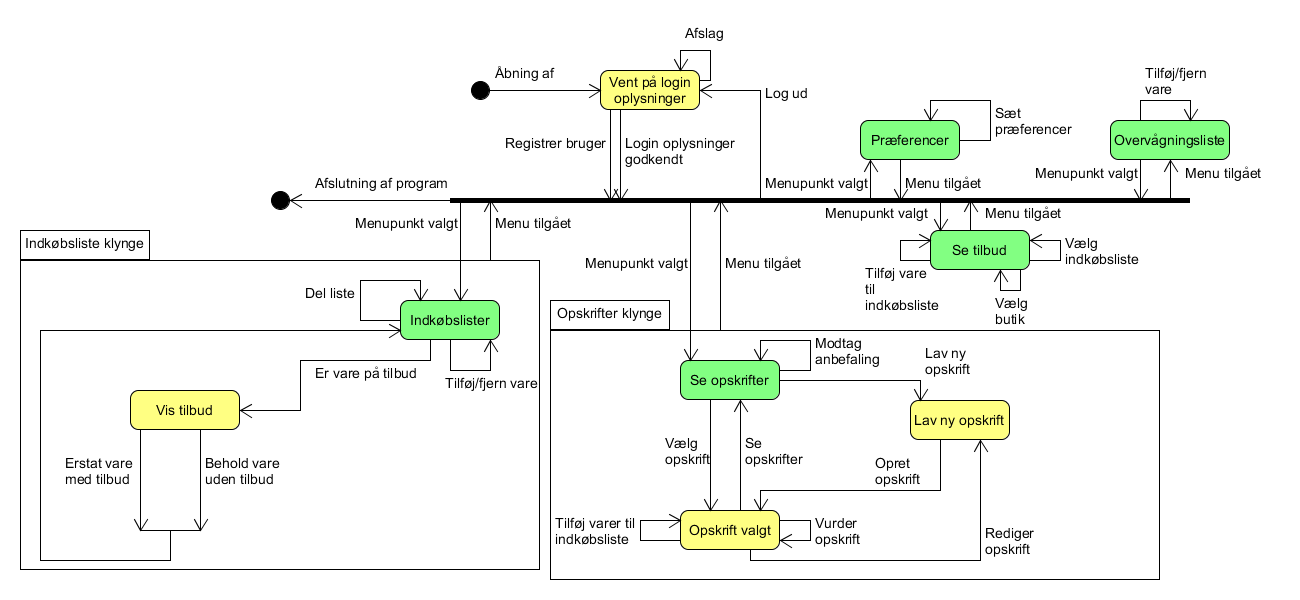
\includegraphics[scale=0.6, angle=90]{images/Diagrams/Tilstandsdiagram.PNG}
	\caption{Tilstandsdiagram for systemet}
	\label{tilstandsdiagram}
\end{figure}

Tilstandsdiagrammet, \myref{tilstandsdiagram}, viser de forskellige stadier systemet kan være i, samt hvilke funktionaliteter der er tilgængelige fra disse stadier.
Diagrammet hjælper med at danne overblik over navigeringen i systemet, og hvilken proces der opstår under udførelse af diverse brugsmønstre.
Markeret med grønt, ses de fem hovedmenuer.
Efter en bruger er logget ind, kan disse hovedmenuer til hver en tid tilgås.
Menuen er repræsenteret gennem den længere sorte centerlinje,  alle pile der går ind her, giver adgang til alle de pile der går ud, pilene repræsenterer en hændelse igangsat af brugeren.
En klynge kan til hver en tid uanset tilstand, tilgå hændelser der går ud af klyngens boks, herfra kan man således se, at menuen altid er tilgængelig, såvel som logud funktionen.

Indikeret med pile, kan man se hvilke funktionaliteter der er tilgængelig fra en given tilstand, samt om disse er sekventielle eller iterative hændelser.
En sekventiel funktion skifter tilstanden på systemet, mens en iterativ blot opdaterer systemets information, mens den forbliver i tilstanden.
Eksempelvis har den grønne menu-boks \textit{Præferencer} en iterativ funktion på sig, da denne blot opdaterer information i systemet, frem for at skifte tilstand i modsætning til funktionen \textit{Vælg opskrift}, som er sekventiel.
Hvis brugeren fra menuen \textit{Se opskrifter} giver brugerinputtet \textit{Vælg opskrift} følges sekvensen til en ny tilstand \textit{Opskrift valgt} Herfra åbnes således op for nye funktionaliteter for brugeren.
Hele diagrammet følger disse to typer af hændelser, som er gældende for alle tilstande og funktioner.



\subsection{Funktioner}\label{subsec:funktioner}

I dette afsnit beskrives funktionerne der skal bruges for at kunne håndtere hændelserne fra problemområdet, og brugsmønstrene beskrevet ovenfor.
Der findes fire typer funktioner: Aflæsnings-, opdaterings-, beregnings-, og signaleringsfunktioner.\citep{OOA&D2001}
Først identificeres funktionerne, hvorefter der gives en kategori til funktionerne, og en bedømmelse af deres kompleksitet. Herefter gives en kortfattet beskrivelse af funktionen hvor dette er tilstrækkeligt, ellers gives en dybere beskrivelse.

På figur \ref{tabel:functionstable} ses en tabel over de forskellige funktioner smat deres kompleksitet og kategori.
Kategorien beskriver hvilke type handling funktioner udfører og  kompleksistetssøjlen beskriver hvor kompleks en given funktion er, dette fastsættes på baggrund af om en given funktion har mere end en kategori, samt en vurdering af hvor kompleks funktionens arbejde er.
\begin{table}[H]
  \centering
    \colorlet{shadecolor}{gray!40}
    \rowcolors{1}{white}{shadecolor}
      \begin{tabular}{l|lllll}
      %\hline
      \textbf{Funktioner}			& {Kompleksitet}	& {Kategori}  	\\ \hline
      Log ind						& Medium			& Beregning, Opdatering		\\
      Log ud						& Simpel			& Opdatering	\\
      Registrer bruger				& Simpel			& Opdatering	\\
      Tilføje varer til lister		& Simpel       		& Opdatering	\\
      Fjerne varer fra lister		& Simpel       		& Opdatering	\\
      Oprette og slette lister		& Simpel       		& Opdatering	\\
      Dele lister					& Medium       		& Opdatering	\\
      Søgning på tilbud for varer   & Medium     		& Beregning		\\
      Sætte præferencer				& Simpel       		& Opdatering	\\
      Filtrere for præferencer		& Kompleks     		& Beregning		\\
      Give vurdering				& Simpel       		& Opdatering	\\
      Sende anbefaling				& Meget kompleks	& Aflæsning, signalering, beregning		\\
      Meddele tilbud på varer		& Medium      		& Signalering	\\
	    Se opskrifter					& Simpel       		& Aflæsning		\\
      Oprette opskrift      & Simpel          & Opdatering  \\
      Ændre opskrift        & Simpel          & Opdatering \\
      Kopier opskrift       & Simpel          & Opdatering \\
	    Se tilbud						& Simpel       		& Aflæsning		\\
      Hente tilbud					& Simpel	       	& Opdatering	\\
    \end{tabular}
  \caption{Funktionstabel. Viser de forskellige funktioner der skal bruges, samt deres kompleksitet og kategori.}\label{tabel:functionstable}
\end{table}

\textbf{Log ind:} Her bliver sendt brugerinformationer, som verificeres med brugerne registreret i systemet.
Hvis dette fuldføres, opdateres modellaget således brugeren er registreret som værende logget ind.

\textbf{Log ud:} Brugeren der før var logget ind, opdateres til at være logget ud.

\textbf{Registrer bruger:} En ny bruger sender sine brugerinformationer, og et nyt login oprettes i modellaget.

\textbf{Tilføje varer til lister:} Denne funktion skal tilføje et objekt af vare klassen til en indkøbsliste, eller en overvågningsliste.

\textbf{Fjerne varer fra lister:} Funktionen her skal så fjerne disse objekter igen.

\textbf{Oprette og slette lister:} Denne funktion bruges når en indkøbsliste skal oprettes således man kan tilføje varer til denne.

\textbf{Dele lister:} Skal opdatere modellaget således en anden bruger kan tilgå samme indkøbsliste som brugeren der deler sin liste.

\textbf{Søgning på tilbud for varer:} Søger efter tilbud som passer til varen der søges for.

\textbf{Sætte præferencer:} Funktionen skal sætte forskellige præferencer som vælges af brugeren, således brugerens oplevelse rettes efter brugerens præferencer.

\textbf{Filtrere for præferencer:} Funktionen skal findes i to udgaver. Der skal være filtrering i forhold til præferencer for både tilbud, og opskrifter.

\textbf{Give vurdering:} Funktionen skal modtage en vurdering fra brugeren og gemme denne i modellaget.

\textbf{Sende anbefaling:} Funktionen her er meget kompleks da der indgår mange forskellige typer handlinger.
Brugerne har vurderet forskellige opskrifter, og der beregnes en anbefaling ud fra disse.
Når anbefalingen er lavet skal den gives eller signaleres til brugeren.

\textbf{Meddele tilbud på varer:} Når en varer på overvågningslisten kommer på tilbud sender denne funktion et signal til brugeren derom.

\textbf{Se opskrifter:} Funktionen skal hente opskrifterne fra modellaget.

\textbf{Se tilbud:} Funktionen henter tilbudene fra modellaget.

\textbf{Hente tilbud:} Denne funktion henter tilbud, vha. API'et fra eTilbudsavis, disse skal derefter gemmes i modellaget.

Denne analyse af funktionerne hjælper med at danne et overblik over hvilke funktionaliteter der skal designes, samt hjælper det til at stille krav til det systemet.
I det følgende afsnit stilles der krav til systemet.
